\chapter{Implementierung}
Bei der Konzeptionierung wurden Punkte wie die Parametereinstellungen, die Ameisenkolonie als zentraler Punkt der Applikation, sowie die Ameise als einzelner Akteur beschrieben. Auch wurden Begriffe wie die SOLID-Prinzipien aufgezeigt und die Umsetzung beschrieben. Ebenso wurde für ein Beispiel des Ablaufs der Applikation ein numerisches Beispiel berechnet. Im Folgenden wird auf die wirkliche Umsetzung der einzelnen Punkte eingegangen, sowie auch der Arbeitsablauf der letztendlichen Implementierung beschrieben. Als Beweis der Funktionsfähigkeit werden zwei Beispiele zur Berechnung herangezogen.


%Als Beweis der Funktionsfähigkeit werden zwei Beispiele berechnet: 
%\begin{itemize}
%	\item numerisches Beispiel aus Kapitel \ref{numerschiesBeispiel}
%	\item die Problemstellung des ``a280 drilling problem''
%\end{itemize}

\section{Beschreibung der Implementierung}
Um die Funktionsweise der Softwarelösung zu verstehen, ist eine klare Übersicht über die einzelnen Bestandteile notwendig. Diese wird im Folgenden über ein Klassendiagramm inkl. Beschreibung gegeben. Danach werden noch die einzelnen Abschnitte in ihrer Funktion beschrieben.

\subsection{Klassendiagramm}
Bevor auf den genauen Funktionsablauf der Applikation eingegangen wird, sollte zuerst ein Überblick auf die Implementierung gegeben werden. Hierzu ist in Abbildung \ref{classDiagram} der komplette Umfang aller Klassen aufgezeigt
\footnote{Aus Gründen der Übersichtlichkeit wurden die getter- und setter-Methoden weggelassen, um die Abbildung nicht über zu dimensionieren}. Leicht erkennbar ist, dass der größte Teil der Logik innerhalb des aco-Pakets - welches unter anderem Ant und Colony enthält - stattfindet. Landscape, also die Klasse welche das \ac{TSP} beschreibt, dient nur als Schnittstelle zur Abfrage der Distanzen zwischen den Städten.

\begin{figure}[h]
	\centering
	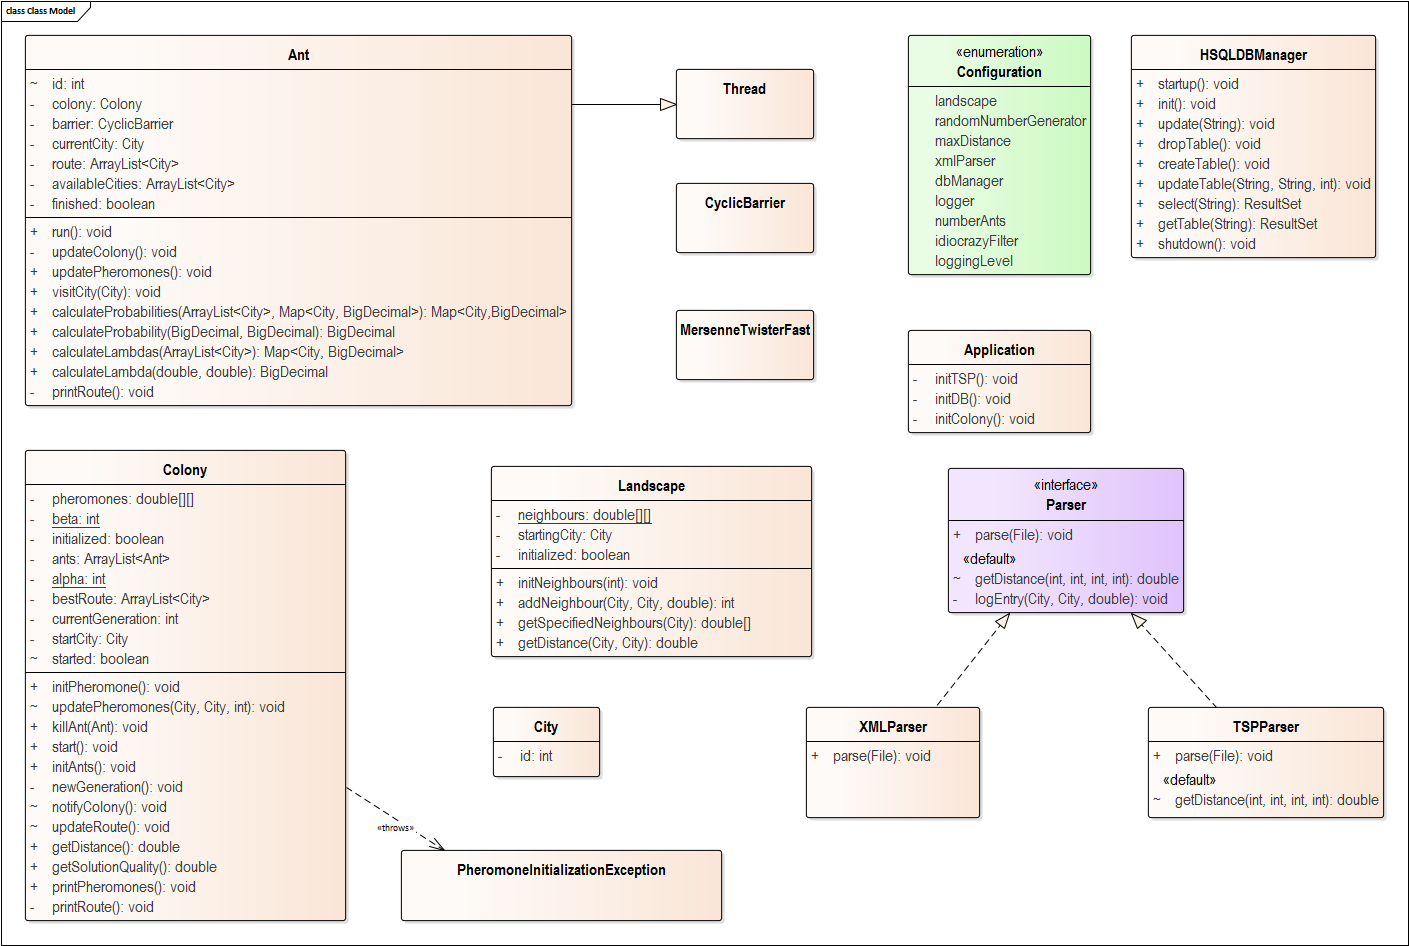
\includegraphics[width=\linewidth]{../../../01_uml/classModel.png}
	\caption{Klassendiagramm der vorliegenden Softwarelösung}
	\label{classDiagram}
\end{figure}

\subsection{Persistenz}
Um die Ergebnisse der einzelnen Generationen persistent abspeichern zu können, ohne den Speicherverbrauch des Programms ansteigen zu lassen, wird eine Datenbank-Anbindung an eine HSQLDB-Datenbank verwendet. Um die Performance möglichst hoch und den Datenbankumfang möglichst klein zu halten, werden in dieser allerdings nur zwei Tabellen erstellt und verwaltet.

Zum Einen wird von jeder Generation, welche den Algorithmus durchlaufen hat, die beste Route erfasst und abgespeichert. Hierbei besteht ein Tabelleneintrag lediglich aus einer Zufalls-ID, der Route als String und der Distanz als Double. 

Zum Anderen wird eine Tabelle zur Verfolgung der Verbesserung angelegt. In der Historie wird eine Route nur dann abgespeichert, wenn diese sich im Vergleich zur vorherigen auch verbessert hat. Somit besteht diese aus den gleichen Attributen, wie die Generationen-Tabelle, mit dem Zusatz, dass auch die Generation, welche die Verbesserung verursacht hat, mit einer Ganzzahl abgespeichert wird.

\subsection{Applikation}
Dem Bereich der Applikation sind im Grund zwei Klassen zu zu ordnen: die Applikation selbst, sowie die Konfiguration. Hierbei ist die Konfiguration für alle Klassen und Instanzen innerhalb des Programms erreichbar und enthält alle Konfigurationen, sodass diese zentral angepasst werden können. 

Auch wird über die Konfiguration der Logger angesprochen, sodass hierzu keine eigene Klasse notwendig wird. Die Applikation hat als einzigen Zweck die Problemstellung einlesen zu lassen, sowie die Architektur zu initialisieren, um diese dann zu starten. Nachdem die Kolonie gestartet ist, wartet die Applikation nur noch darauf, die Datenbank wieder schließen zu dürfen.

\subsection{TSP}
Der \ac{TSP}-Bereich der Architektur dient zu aller erst der Verdeutlichung des Aufbaus. So soll durch die Verwendung der City-Klasse statt einfachen Integern das Verständnis gefördert werden. Innerhalb der Landscape-Instanz - welche in der Konfiguration zentral initialisiert wird -  wird die zweidimensionale Matrix der Distanzen zwischen den Städten bereit gehalten. 

Über diese Matrix kann immer zentralisiert der Wert von den Ameisen nachgefragt werden, ohne eine unnötige Berechnung durchzuführen. Ebenso fördert dieser Aufbau die Sicherung der Funktionsfähigkeit, da einfacher sichergestellt werden kann, dass die Distanzen richtig berechnet werden. Ein weiterer Vorteil ist, dass die Ameisen hier eine Liste von Nachbarn der derzeitigen Position nachfragen können, indem sie ihren derzeitigen Standort übergeben. Dies vereinfacht das Konzept bei der Berechnung innerhalb der Ameisen-Klasse.

\subsection{ACO}
Der hauptsächliche Teil der Berechnung wird innerhalb des \ac{ACO}-Bereichs durchgeführt. Denn hier befindet sich die Ameisenkolonie, als Verwaltungsorgan, und die Ameisen, welche als Threads gleichzeitig auf die Suche nach der bestmöglichen Lösung gehen.

Von der Kolonie werden die Ameisen insofern verwaltet, dass die Threads über diese Klasse gestartet werden, sowie hier auch die Ergebnisse abgeliefert werden. Nach jeder Generation wird innerhalb der Kolonie für jede Ameise eine Auswertung gestartet, ob die Route besser war als die derzeit beste. Sollte dies der Fall sein, wird die alte Route mit der neuen Route überschrieben.

Unabhängig davon ob eine neue beste Route gefunden wurd oder nicht, wird nach jeder Generation von Ameisen ein Update auf die Pheromonmatrix durchgeführt. Hierbei meldet jede Ameise für jeden Weg, den sie zwischen zwei Städten gegangen ist, einen Wert, welcher auf den derzeitigen Pheromonwert addiert werden soll. Hierfür iteriert eine Ameise über die Route, welche sie sich gemerkt hat, und ruft die updatePheromone-Methode der Kolonie auf, mit dem Wert $1/distance$, wobei $distance$ der Distanz zwischen der Stadt, über welche gerade iteriert wird, und der Folgestadt beträgt. 

Die restliche Berechnungsarbeit wird von den einzelnen Ameisen bzw. Threads bewältigt. Diese berechnen ab dem Startpunkt für alle möglichen Nachbarn
\footnote{Ein Nachbar ist dann erreichbar, wenn dieser noch nicht in der Route vorgekommen ist, also noch nicht besucht wurde.} einen $\lambda$-Wert\footnote{Beschrieben wurde diese Berechnung bereits in Kapitel \ref{parameter}}. 
Als nächstes werden alle $\lambda$s aufsummiert, um mit den einzelnen $\lambda$s der Städte dividiert durch die Summe die Wahrscheinlichkeit zu berechnen. Hierdurch wird beschrieben, dass Städtepaare, welche eine kurze Distanz besitzen, sowie einen hohen Pheromonwert besitzen, deutlich wahrscheinlicher besucht werden. Hierbei kann eine unterschiedliche Gewichtung vorgenommen werden, wie in Kapitel \ref{parameter} und Kapitel \ref{analyse} beschrieben wurde.

Nachdem für alle erreichbaren Städte die Wahrscheinlichkeiten berechnet wurden, wird eine Zufallszahl bestimmt. Sollte eine Wahrscheinlichkeit für eine Stadt höher sein, als die Zufallszahl so wird die Berechnung an dieser Stelle beendet und die Ameise besucht diese Stadt. Sollte diese Bedingung für keine einzelne Stadt erfüllt werden, so werden die Wahrscheinlichkeiten solange aufsummiert bis die Summe größer ist als die Zufallszahl. Die Stadt, bei welcher diese Schwelle überschritten wird, wird dann von der Ameise aufgesucht.

Sobald jede Ameise ihre Route beendet hat und wieder bei der Anfangsstadt angekommen ist, wird über die CyclicBarrier zentral eine Methode innerhalb der Kolonie angestoßen. Diese fordert nach und nach jede Ameise auf, das Ergebnis zu melden, um die Pheromonmatrix zu aktualisieren. Nachdem die Kolonie vollständig aktualisiert wurde, ist die derzeitige Generation beendet und es wird eine neue generiert und gestartet.
\section{Beschreibung der verwendeten Datenstrukturen}
Nachdem nun die logischen Schritte der Implementierung aufgezeigt wurden, folgt ein kurzer Ausblick auf die Auswahl der verwendeten Datenstrukturen. Hierbei wird auch eine Einschätzung auf die Effizienz dieser Datenstrukturen gegeben und die Entscheidung, welche Datenstruktur verwendet wird, begründet.

\subsection{BigDecimal}
Eine Besonderheit der vorliegenden Implementierung ist die Verwendung von BigDecimal statt Double als zentrale Zahlenwerte. Hierbei werden BigDecimal vor allem dann verwendet, wenn die Berchnung der Lambda- bzw. Wahrscheinlichkeitswerte durchgeführt werden muss. Hier hat sich schnell gezeigt, dass der Zahlenraum von Double\footnote{4,94065645841246544E-324 bis 1,79769131486231570E+308 \cite{Ullenboom2011}} bzw. auch die Implementierung von Double selbst nicht genau genug ist, um mit extrem kleinen Werten arbeiten zu können. Diese extrem kleinen Werte werden in der Applikation dann erreicht, wenn ein recht hoher Gewichtungswert gewählt wird, welcher zu einer hohen Potenzierung führt. Da die Applikation aber unabhängig der Gewichtung immer zuverlässig und genau arbeiten soll und muss, ist dieser Zustand nicht haltbar.

Um dieses Problem zu lösen, wurden BigDecimal als Ausweg gewählt. BigDecimal-Zahlen werden nicht zwingend als einzelner Speicher allokiert. Dies hat den Vorteil, dass eine beliebig genaue Genauigkeit erzeugt werden kann, da die Nachkommastellen nicht begrenzt werden durch einen maximalen Wert, wie bei primitiven Datentypen. Der Nachteil dieser Vorgehensweise ist ein Overhead, den das System verwalten muss, welcher bei primitiven Datentypen nicht vorhanden ist. Allerdings ist dieser Overhead, falls Genauigkeit wichtig ist, immer einer ungenauen Arbeitsweise vorzuziehen.

\subsection{ArrayList}
ArrayList ist eine gängige Datenstruktur in Java, wie auch in wie vielen anderen Programmiersprachen\footnote{In anderen Sprachen heißt die Datenstruktur zwar anders, hat aber meist die selbe Arbeitsweise.} Sie hat den Vorteil, dass bei Erstellung der Liste nicht klar sein muss, wie lang die Liste werden wird. Dadurch kann die Liste dynamische bearbeitet werden, indem immer Objekte hinzugefügt und entfernt werden können. Wie immer gibt es aber nicht nur Vorteile. 

Ein großer Nachteil von ArrayList ist der unperformante Speichervorgang der Daten. Da nicht bekannt ist, wie lange die Liste wird, kann auch kein zusammenhängeneder Speicher allokiert werden. Dies bedeutet, dass die Daten in der Liste meist fragmentiert abgespeichert werden müssen. Dadurch wird die Performance eingeschränkt, da zwischen den Daten immer die Pointer-Referenz aufgelöst werden muss. Bei Arrays ist dies nicht der Fall. Denn hier würde ein einziger Block an Daten belegt werden, über den in einem Zug iteriert werden kann. Somit ist eine Nutzung von Arrays generell der einer ArrayList vorzuziehen, solange die Größe bekannt ist. 

Ein weiterer Nachteil ist der Struktur einer ArrayList geschuldet. Wenn eine ArrayList erstellt wird, belegt diese ein Array in welchem die zu speichernden Objekte abgelegt werden. Sollte das Array während der Laufzeit zu klein werden, muss ein neues Array belegt werden und das alte kopiert werden. Dies verursacht wiederum einen Performance-Einbruch bei der eigentlichen Applikation.\footnote{vgl. \cite{Smyth2007}}

Im vorliegenden Fall wurden ArrayList vor allem benutzt, um die möglichen erreichbaren Nachbarn abzuspeichern. Man könnte über einen Zähler und die Länge der Distanzmatrix zwar einen Algorithmus implementieren, welcher die nötige Länge berechnet und damit ein Array erzeugt. Allerdings wäre dies zum Einen umständlich und zum Anderen unschön. Auch würde der Performance-Gewinn relativ klein ausfallen, da bei jedem Schritt die Berechnung durchgeführt werden muss. Generell würde die Wartbarkeit des Codes darunter leiden. Um diese Punkte zu vermeiden wurde ArrayList als standardisierte Datenstruktur verwendet, um trotz allem eine möglichst performante und speichereffiziente Arbeitsweise in allen Methoden zu gewährleisten.

\subsection{HashMap vs zweidimensionales Array}
Zu Beginn der Implementierung wurden die Möglichkeiten zur Darstellung der Distanzen und Pheromonwerte betrachtet. Da alle Städte untereinander vernetzt sind, gibt es für jeden Pfad jeweils einen Distanzwert und einen Pheromonwert. Somit ergibt sich immer eine zweidimensionale Matrix. Der logische Schritt wäre diese Matrix über ein zweidimensionales Array zu implementieren. Allerdings wäre auch eine Implementierung über eine HashMap möglich. Um die beiden Möglichkeiten auszuloten wurden mehrere Aspekte beachtet:
\begin{itemize}
	\item Performance
	\item Übersichtlichkeit
	\item Umständlichkeit
\end{itemize}
Der Punkt der Performance ist relativ schnell abgehandelt. Denn ähnlich zur ArrayList arbeitet auch eine HashMap mit einem Array als "Backend". Somit kann eine HashMap nicht schneller als ein Array sein. Dennoch kann es Anwendungsfälle geben, in denen es sinnvoller ist eine HashMap zu verwenden.

Ein möglicher Anwendungsfall wäre zum Beispiel, wenn durch eine HashMap eine bessere Übersichtlichkeit gewährleistet wäre. Denn in einem Array können immer nur Integer-Werte als Referenzen gewählt werden, bei einer HashMap aber auch ein beliebiges Objekt. Dadurch ist im objektorientierten Umfeld ein besseres Verständnis gewährleistet. Dies ist auch der Grund, warum zu Beginn die HashMap ausgewählt wurde, um Distanz- und Pheromon-Werte abzuspeichern. Da diese Werte immer in Beziehung zwischen zwei Städten stehen, wäre es auch sinnvoll diese beiden Städte als Referenz zu benutzen. Dies wäre bei einem Array nicht ohne weiteres möglich.

Der letzte Punkt der beachtet wurde war die Umständlichkeit. Auch wenn eine HashMap deutlich sinnvoller und übersichtlicher erscheint gibt es wieder einen Nachteil. Man kann nicht ohne weiteres der Reihe nach über alle Einträge iterieren. Auch kann nicht ohne weiteres ein Ausschnitt aus einem Array übergeben werden. Bei einem Array kann eine einzelne Spalte zurückgegeben werden, was zum Beispiel bei der Abfrage der Nachbarn einer Stadt sinnvoll ist. Im Falle einer HashMap müssten alle Einträge durchlaufen werden und geprüft werden, ob die derzeitige Stadt in dem Key-Paar als erste Stadt eingetragen ist.
Dies führt zum Einen zu schlechterer Code-Qualität und zum Anderen zu Performance-Verlusten, da die ganze HashMap durchlaufen werden muss.

Vor allem wegen der Umständlichkeit wurde relativ schnell von einer Struktur mittels HashMaps auf einen, auf zweidimensionalen Arrays basierenden, Aufbau gewechselt.


\documentclass[a4paper, 12pt, oneside]{scrbook}
\usepackage{fancyhdr}

\begin{document}
	
	\title{Test}
	\maketitle

	\chapter{Inhalt...}
		\thispagestyle{fancy}
	Inhalt...
\end{document}
\section{Beweis der Funktionsfähigkeit}
In der Theorie funktionierte dieses Konstrukt bereits in Kapitel \ref{architektur}. Im Folgenden soll gezeigt werden, dass das entworfene Konstrukt aber auch in der Praxis relevante Werte liefert. Hierzu wird das in Kapitel \ref{numerschiesBeispiel} herangezogen, sowie ein standardisiertes Beispiel aus dem Themenbereich des \ac{TSP}, nämlich das a280-Problem - also eine Problemstellung mit 280 Städten.

\subsection{numerisches Beispiel}
In Abbildung \ref{tspAcoNumerisch} in Kapitel \ref{numerschiesBeispiel} wurde der Aufbau des numerischen Beispiels schon gezeigt. An der Ausgabe, welche beispielhaft in Abbildung \ref{numerischBeweis} als Ausschnitt der Log-Datei gezeigt ist, ist gut zu erkennen, dass schnell eine optimale Strecke gefunden werden konnte. 

Als Erinnerung: Bei der manuellen Berechnung des numerischen Beispiels belief sich die optimale Route auf eine Distanz von 29. Diese trat bei drei Ameisen nach drei Generationen auf. Zu Testzwecken lief das Programm nur mit einer Ameise, da bei einer zu hohen Anzahl an Ameisen bereits die erste Generation die optimale Strecke fand. Es lässt sich hiermit ableiten, dass die implementierte Architektur genauso abläuft wie das theoretische Konzept, wodurch eine fehlerfreie Implementierung bewiesen ist.

\begin{figure}[H]
	\centering
	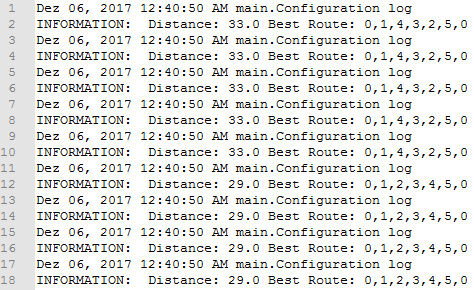
\includegraphics[width=0.6\linewidth]{images/numerischErgebnis.png}
	\caption{Ausschnitt der Log-Datei bei der Berechnung des numerischen Beispiels aus \ref{numerschiesBeispiel}. Jede Log-Zeile steht hier für eine Generation an Ameisen.}
	\label{numerischBeweis}
\end{figure}



\subsection{a280 drilling problem}
Aber nicht nur die fehlerfreie Implementierung soll bewiesen werden, sondern auch die Anwendungsmöglichkeiten auf komplexe Problemstellungen. Ohne diese Möglichkeit wäre das Programm darauf beschränkt die optimale Strecke innerhalb des numerischen Beispiels zu finden. Durch Abbildung \ref{drillingBeweis} lässt sich aber beweisen, dass auch deutlich größere Probleme sich berechnen lassen. Erkennbar sind mehrere Punkte:
\begin{itemize}
	\item Die Berechnungszeit wird etwas höher, erkennbar an dem Log-Zeitraum, der nun drei Sekunden umfasst
	\item Die Berechnungszeit beträgt immer noch deutlich weniger als eine Sekunde
	\item Es findet eine stetige Verbesserung der Distanz statt
\end{itemize}
Zusätzliche zu den Punkten lässt sich noch eine weitere Aussage ableiten: Das Problem lässt sich berechnen. Hierdurch ist der Punkt, der eigentlich bewiesen werden sollte, nachweislich belegt. Noch nicht bewiesen ist, ob der Algorithmus auch in kurzer Zeit ein Optimum finden kann. Da dieser Beweis allerdings mehr Hintergrundwissen und mehr Nachweise erfordert, wird dieser im späteren Kapitel \ref{proofOfConcept} behandelt.

\begin{figure}[H]
	\centering
	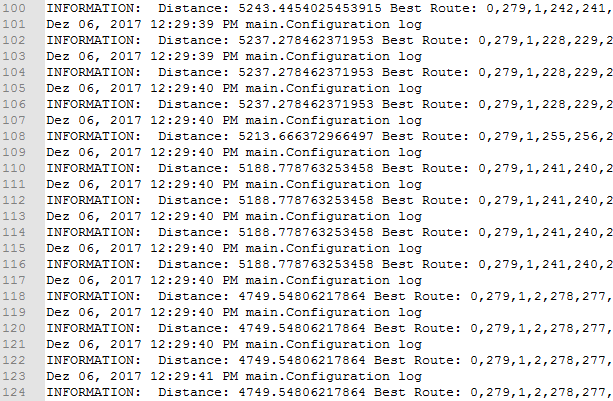
\includegraphics[width=0.6\linewidth]{images/a280Ergebnis.png}
	\caption{Ausschnitt der Log-Datei bei der Berechnung des ``a280 drilling problem''. Auch hier steht jede Log-Zeile für eine Generation an Ameisen.}
	\label{drillingBeweis}
\end{figure}
%\section{Vergleich der Auswirkung der Parametergewichtung}

\section{Performance-Analyse}
Selbstverständlich ist für eine richtige Implementierung nicht nur wichtig, dass diese funktioniert. Sie muss dies auch möglichst performant und effizient tun. Hierzu werden mehrere Testläufe in Hinblick auf die Performance durchgeführt. Im Folgenden werden diese Testfälle beschrieben, sowie auch die Hardware, auf welcher die Tests durchgeführt werden. Ohne die Referenz zur verwendeten Hardware wäre eine Aussage über die Performance nur sehr bedingt verwendbar. In Abbildung \ref{hardware} sind die relevanten Komponenten aufgelistet. Zu beachten ist hierbei, dass AMD-Prozessoren allgemein eine höhere Multithreading-Performance besitzen, welche in der vorliegenden Software genutzt wird.
\begin{table}[H]
	\centering
	\setstretch{0.75}
	\begin{tabular}{c c c c c c c}
		Komponente & Name & Technische Daten\\
		CPU & AMD FX8350 & 8 Kerne, 4.2 GHz\\ 
		RAM & Kingston 99U5471 & 24 GB DDR3, 666 MHz  \\ 
	\end{tabular}
	\caption{Für Performance-Benchmarks verwendete relevante Hardware}
	\label{hardware}
\end{table}
Als Grundlage der Benchmarks wird das a280-\ac{TSP} verwendet um zum Einen eine standardisierte Grundlage zu erhalten und zum Anderen um eine genügend große Problemstellung zu erzeugen, die bezogen auf den Rechenaufwand auch relevant ist. Es wurden 8 parallele Threads gestartet, um eine hohe Auslastung der Hardware zu gewährleisten, ohne durch zu umfangreiches Threadhandling Performance einzubüßen. Die Applikation wurde genau 60 Sekunden lang betrieben, um einen einfachen Vergleichswert zu erhalten.

\newpage
\subsection{CPU-Auslastung}
Wie in Abbildung \ref{cpuUsage} zu sehen ist, beansprucht die Applikation durchgehend zwischen 60 und 70 Prozent. Dass keine 100 Prozent genutzt werden können, liegt daran, dass die Test-Umgebung nicht optimal ist. So wurden die Benchmarks auf einem Desktop-PC in normalen Betrieb mit gleichzeitiger Heim-Nutzung durchgeführt. Da für das Betriebssystem keine Priorisierung der Applikation vorliegt, wird diese mit anderen Programmen gleichgestellt und die Ressourcen auch dementsprechend verteilt.

\begin{figure}[h]
	\centering
	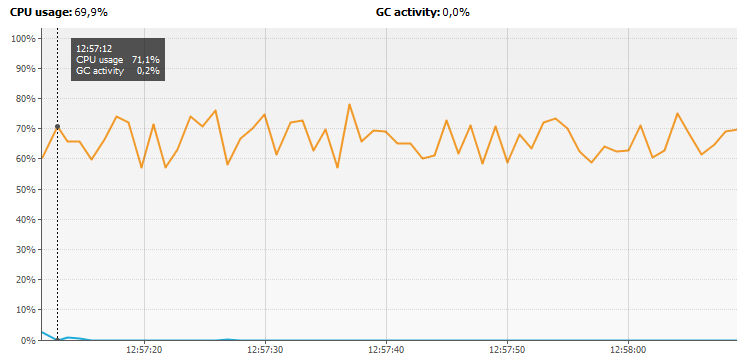
\includegraphics[width=0.9\linewidth]{images/cpuUsage.png}
	\caption{Aufzeichnung der CPU-Beanspruchung der Applikation über die gesamte Laufzeit}
	\label{cpuUsage}
\end{figure}

Würde die Applikation auf einer einwandfreien Test-Umgebung betrieben werden, würden bis zu 100 Prozent der CPU genutzt werden, was zu einer Verbesserung der Performance führen würde. Aber eine hohe Nutzung der CPU alleine kann nicht beschreiben, wie effizient ein Programm arbeitet. Hierzu sind noch andere Parameter notwendig, wie zum Beispiel die Nutzung des Hauptspeichers.

\subsection{Heap-Nutzung}
In Abbildung \ref{heapUsage} ist eine Statistik des benötigten Heaps der Applikation über die Laufzeit zu sehen. In blau markiert ist der benötigte Speicher im Heap zu einem bestimmten Zeitpunkt. In orange hinterlegt ist die Menge an Speicher, welche vom Programm allokiert wurde. Es lassen sich hierbei mehrere Aussagen ableiten. 

Zum Einen ist die Speicherallokierung konstant. Es werden vom Programm immer 2,4 GB an RAM belegt. Zum Anderen ist der Unterschied zwischen belegtem und allokierten Speicher teilweise enorm, was aber nicht auf die Arbeitsweise des Programms zurückzuführen ist. Zusätzlich lässt sich über die Grafik auch noch bestätigen, dass der GarbageCollector von Java zuverlässig nicht mehr benötigte Strukturen im Heap wieder frei gibt, was durch die lokalen Tiefpunkte im Heap-Verbrauch ersichtlich wird.

\begin{figure}[h]
	\centering
	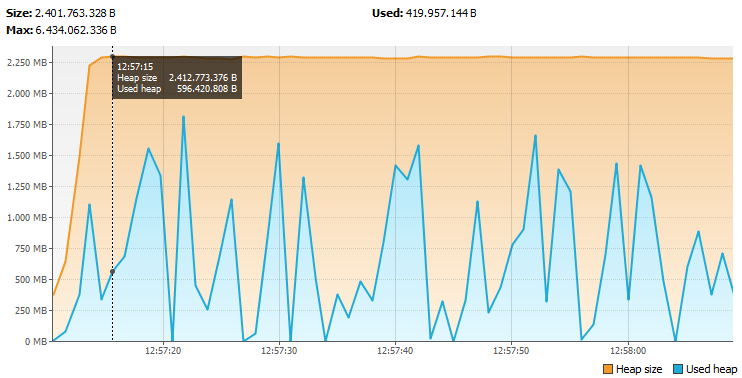
\includegraphics[width=0.9\linewidth]{images/heapUsage.png}
	\caption{Aufzeichnung des Speicherverbrauchs der Applikation über die gesamte Laufzeit. Blau markiert ist der derzeit verwendete Speicher, in orange der allokierte Speicher.}
	\label{heapUsage}
\end{figure}

Als möglichen Optimierungspunkt lässt sich hier der überdimensionierte Heap nennen. Mit 2,4 GB ist der Verbrauch zwar nicht so hoch, dass er eine Verwendung auf einer heutigen Hardware verhindert. Allerdings ist bei einem Anspruch einer möglichst effizienten Software dieser unnötige Verbrauch nicht haltbar.

\subsection{Anzahl Threads pro Minute}
Schlussendlich ist nicht die Auslastung der Hardware ausschlaggebend für die Performance eines Algorithmus, sondern wie effizient dieser rechnet. Als Richtwert kann in diesem Beispiel die Anzahl an Threads pro Minute herangezogen werden, da ein Thread einem Rechenschritt entspricht bzw. über die Anzahl an Threads auch die Anzahl an Generationen errechnet werden können. Die Anzahl an Generationen ist hierbei ein direkter Richtwert wie viele Routen abgelaufen werden konnten.

In Abbildung \ref{threadUsage} ist eine Statistik der in der Applikation aktiven Threads aufgezeigt. In blau werden die Daemon-Threads - hauptsächlich Systemthreads, wie beispielsweise der GarbageCollector - und in rot die Live-Threads gezeigt. Die Menge an aktiven Live-Threads beläuft sich im Durchschnitt auf 19. Für die Berechnung werden pro Generation acht Threads gestartet, welche nach der Generation auch wieder abgebaut werden. Somit ist auch hier wieder ein Overhead vom System vorhanden - in Summe 11 Live-Threads und 10 Daemon-Threads.

\begin{figure}[h]
	\centering
	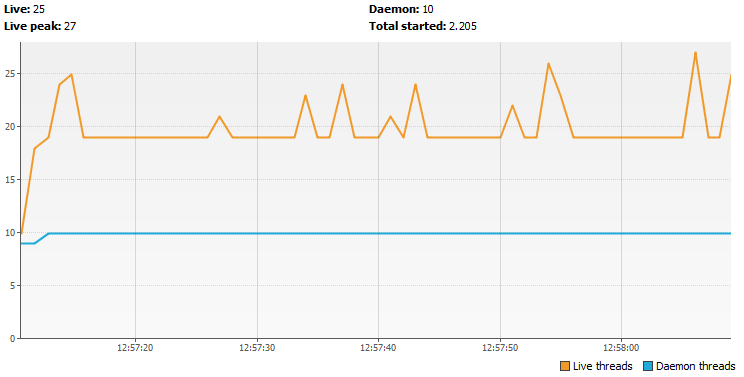
\includegraphics[width=0.9\linewidth]{images/threadUsage.png}
	\caption{Aufzeichnung der Menge an gleichzeitig aktiven Threads des Programms. In blau gezeichnet ist die Menge an Daemon-Threads, in orange die Anzahl an aktiven Live-Threads.}
	\label{threadUsage}
\end{figure}

Mithilfe der Datenerfassung lässt sich auch die genaue Anzahl an gestarteten Threads innerhalb der Applikation ermitteln. Innerhalb von 60 Sekunden wurden 2170 Threads bzw. Ameisen gestartet. Somit wurden ca 36,1 Ameisen pro Sekunde generiert. Teilt man diese Menge durch die Anzahl an Ameisen pro Generation (also acht) erhält man die Menge an Generationen pro Sekunde - in diesem Fall ca. 4,5.

\newpage
\subsection{Fazit zur Performance}
Nun wurden im Detail die relevanten Daten zur Performance genannt und analysiert. Als Fazit können einige Punkte genannt werden:
\begin{itemize}
	\item Die CPU wird fast vollständig genutzt
	\item Der Heap-Verbrauch ist akzeptabel, aber nicht optimal
	\item Es werden bei acht gleichzeitigen Ameisen 4,5 Generationen des a280-Problem pro Sekunde berechnet
\end{itemize}
Diese Aussagen ergeben eine relativ gute Bewertung der Applikation in Hinblick auf die Performance. Allerdings wurden bereits Schwachstellen erkannt. So ist die Belegung des Speichers im Vergleich zum wirklichen Verbrauch teilweise sehr hoch. Auch entsteht durch System-Threads ein recht großer Overhead. Im weiteren Entwicklungsverlauf dieser Applikation sollte in diesen Punkten noch eine Optimierung vorgenommen werden.

%\section{Vergleich einer Auswahl von möglichen Parametern}
%\section{Paket-Diagramm}{
	
}
%\section{ER-Diagramm}{
	
}